\section{ATLAS Detector}
%ATLAS detector
There are seven experiments around the circumference of the LHC located at the interaction points of the beams: four large experiments called CMS, ALICE, LHCb, and ATLAS as well as three small experiments called TOTEM, MoEDAL, and LHCf.
This thesis uses data collected by the ATLAS (A Large Toroidal Lhc ApparatuS) detector.
ATLAS is a multipurpose particle detector designed to maximize acceptance and precision in order to discover and study new particles.
The experiment has a cylindrical geometry 46~m in length and 25~m in diameter.
The experiment is located at p1 on the LHC ring, and is constructed to cover nearly the entire solid angle surrounding the colliding beams. \cite{atlasFacts}

The detector subsystems perform a variety of tasks.
These range from measuring charge tracks left by particles, along with their energy and momentum.
Some detectors specialize in precisely recording the effects of particles (hits), while others focus on quickly identifying patterns of interest for analysis (triggers).

Throughout the design of the various systems, a key concern is the amount (or budget) of material that each introduces.
Particles may loose energy, be absorbed, or produce secondary particles through interactions as they pass through these materials.
With few exceptions, it is advantageous to reduce the total material that particles pass through.

\begin{figure}[h!]
\captionsetup[subfigure]{position=b}
\centering
\subfloat[][]{{\includegraphics[width=0.5\textwidth]{figures/experiment/atlas/atlasLayout.jpg}}}
\caption{From \url{https://cds.cern.ch/record/1095924}}
\label{fig:atlasLayout}
\end{figure}

Four systems comprise the experiment and serve separate purposes in the measurement of particles leaving the collisions.
The ATLAS magnet system immerses the detector in a strong magnetic field that bends charged particles proportionally to their momentum.
Three cylindrical coaxial systems interact with both charged and neutral particles to collect information.
The first is the inner detector, which precisely measures the tracks of charged particles.
Next, the calorimeters measure the energies of particles.
Finally the muon system helps to identify muons and measure their momentum.
The organization of these systems is illustrated in Figure \ref{fig:atlasLayout}.

This section will describe the design of the experiment, beginning with the four systems that make up the ATLAS.
Following this, the systems for identifying interesting collisions and recording them will be presented.

% Note: principles of detection
% \subsection{Design Philosophy}
\subsection{Coordinate System}

Three coordinate systems are commonly used to describe different aspects ATLAS and its operation. 
A Cartesian coordinate system is defined with its origin at the center of the detector.
The $z$ axis runs parallel to the beamline in the counter-clockwise direction when viewed from above, the $y$ axis points towards the top of the detector, and the $x$ axis points towards the center of the LHC ring.
A cylindrical coordinate system is also defined sharing the same $z$ axis as the Cartesian system.
The azimuthal angle $\phi$ is defined with respect to the Cartesian $x$ axis, and the radius $\rho$ is defined from the $z$ axis.
Since the detector is nearly symmetric under reversing the $z$ axis, it is helpful to refer to the side of the detector with positive $z$ coordinates as the \emph{A side} and the opposite side as the \emph{C side}.
The main body of the experiment, the \emph{Barrel}, is located between the A and C side \emph{end-caps}.
Both of these systems are used in describing the positions of detectors and components within ATLAS.
In particular, the cylindrical system is used to describe the locations of collisions and impact parameter displacements from the beam.

Spherical coordinates are more natural than Cartesian and cylindrical when describing the physical interactions.
This system shares an origin with the previous two systems, and shares the azimuthal angle with the cylindrical system.
The radius $r$ is defined from the center of the detector.
The polar angle $\theta$ is defined with respect to the $z$ axis.
It is common to map polar angles onto \emph{pseudorapidity} defined as $\eta\equiv-\ln(\tan\frac{\theta}{2})$.
The pseudorapidity is conveniently calculated from the longitudinal component \plong of a particle's total momentum $p$ as $\eta=\arctan{\frac{\plong}{|p|}}$.


\subsection{Inner Detector}

\begin{figure}[h!]
\captionsetup[subfigure]{position=b}
\centering
\subfloat[][]{{\includegraphics[width=0.7\textwidth]{figures/experiment/atlas/id.jpg}}}
\caption{Illustration by Joao Pequenao from \url{https://cds.cern.ch/images/CERN-GE-0803014-01}}
\label{fig:atlasId}
\end{figure}

The ATLAS Inner Detector (ID) is the innermost detector system.
Its purpose is to precisely measure the locations of energy deposits left by particles leaving a collision.
To this end, it is comprised of three subsystems: the pixel detector, the silicon-strip tracker, and the transition radiation tracker.
These are shown in Figure \ref{fig:atlasId}.
These are positioned in coaxial cylindrical arrangements around the region of the beam pipe where collisions take place.
The cylinders arrange detectors in a barrel covering $|\eta|<1$ and bookended by two mirrored end-caps.
The total length of the ID is 7~m and the diameter is 2.3~m which enables the full coverage of $|\eta|<2.5$.
The data from the ID subsystems (hits) are used to identify tracks left by particles as they transverse the detector.
In this regard, it is helpful in measuring the impact parameter of particles with a precision that enables the identification of decay products of bottom quarks and tau leptons that travel short distances before decaying.
\cite{pixel}

Both the pixel detector and the silicon-strip tracker belong to the category of solid-state silicon detectors in that they detect ionizing particles through their interaction with a semiconductor.
These use a semiconductor layer doped with an element with an electron affinity (p-type) and a semiconductor layer doped with an electron doner element (n-type).
At the interface between these two layers, electrons equilibrate from the n-type material to the p-type material, producing a \emph{depletion region} and an electric field.
A positive voltage bias is applied to the n-type side of the juncture to expand the depletion region and strengthen the field.
When a charged particle passes through the depletion region, it ionizes atoms liberates electron-hole pairs.
Under the influence of the electric field, these drift to either ends of the depletion region and produce a measurable current.
Drift does not occur outside the depletion region in the absence of an electric field. \cite{grupen}

The first subsystem that particles pass through is the pixel detector.
Here, the silicon is subdivided into a grid of many isolated \emph{pixels} that may be read out individually.
Each pixel is 256~\um thick with a typical surface area of $50\times400\um^2$.
In the barrel, these are grouped into arrays of 24$\times$160 pixels for readout.
Sixteen arrays are housed on a ``module'', which serves the repeating basis of the various pixel layers.
Three layers of detectors are arranged in the barrel with radii of 4~cm, 11~cm, and 14~cm.
In each end-caps, four disks are arranged between $z$=11~cm and $z$=20~cm.
\cite{pixel}
The next subsystem that particles interact with is the silicon-strip tracker (SCT).
The SCT barrel consists of four cylindrical layers, while the end-caps each consist of nine disk layers.
Each barrel layer is built from modules that host two layers silicon wafers divided into lines of microstrips that are 126~mm long and .
In the barrel, the strips are oriented differently depending on their layer, with some running parallel to the beam axes and others offset at an angle of 40~mrad. \cite{sct}

Finally, particles interact with the transition radiation tracker (TRT) positioned outside the SCT.
This is a system of 4~mm diameter gaseous proportional-mode drift tubes.
The tubes, or ``straws'', are made from wound Kapton with a gold-plated 31~\um wire in the center.
The straws are filled with a drift gas mixture of xenon (70\%), carbon dioxide (27\%), and oxygen (3\$).
During operation the Kapton is kept at a -1.5~kV.
When a charged particle passes through a straw, it ionizes the gas and the resulting free electrons drift towards the grounded wire.
The induced current is amplified read out by front end electronics.
The space between the straws is filled with polymer and foil materials so that charged relativistic particles produce transition radiation when they pass through material interfaces.
This is strongest for electrons ($\propto E/m$) and is useful for their identification against pions.
The TRT complements the silicon detectors by providing a large number of tracking points while adding very little to the material budget.
As a result, the 73 layers of tubes are used in the barrel, while 160 layers make up the end-caps.
A charged particle passing through the barrel will produce hits in $\sim30$ TRT straws.
Additionally the fast readout rate of 80-100~kHz compensates for the relatively slow readout possible with the silicon detectors.
\cite{trt} 

In total, 1.5$\times10^{8}$ data channels are read out from the ID with the majority of these coming from the pixel detector.
The ID is used to measure tracks left by muons and electrons, to identify displaced vertices from b-jet decays, and measure to overall momentum expelled from collisions.

\subsection{Calorimeters}

\begin{figure}[h!]
\captionsetup[subfigure]{position=b}
\centering
\subfloat[][]{{\includegraphics[width=0.5\textwidth]{figures/experiment/atlas/calo.jpg}}}
\caption{}
\label{fig:atlasCalo}
\end{figure}

The ATLAS Calorimeter System is comprised of two subsystems: the Liquid Argon Calorimeter (LAr), the Tile Calorimeter.
The LAr is designed to measure energy deposited through electromagnetic interactions.
The Forward Calorimeter is part of the LAr and is positioned in the large-$\eta$ region and provides additional calorimeter coverage.
Wrapped around the exterior of LAr, the Tile Calorimeter is designed to measure the energies of hadronic jets.
Together, these make up the calorimetry system shown in Figure \ref{fig:atlasCalo}.
This is particularly useful in determining the energies of photons and electrons, and to a lesser extent muons.

The calorimeters in ATLAS are divided into electromagnetic and hardonic types.
The electromagnetic calorimeters measure the energy lost by electrons through bremsstrahlung radiation and the energy lost by photons through electron-positron pair production.
Both processes occur at a rate related to the thickness of material that they travel through in term of \emph{radiation length} $X_0$.
\footnote{$X_0\equiv\frac{A}{4\alpha N_AZ^2r_e^2\ln(183Z^{-1/3})}$, where $Z$ and $A$ are the atomic number and weight, $r_e\equiv\frac{1}{4\pi\epsilon_0}\frac{e^2}{m_ec^2}$ is the classical electron radius, $N_A$ is Avogadro's number, and $\alpha$ is the familiar fine structure constant.}
Electrons with energy $E$ loose their energy while traveling through a material per length $x$ at a rate:
\begin{equation}\begin{split}
    -\frac{dE}{dx}=\frac{E}{X_0}.
\end{split}\end{equation} 
Photons undergo pair production with a probability based on their frequency:
\begin{equation}\begin{split}
    -\frac{dw}{dx}=\frac{1}{\lambda_\text{pair}}e^{-x/\lambda_\text{pair}}; \quad \lambda_\text{pair}=\frac{9}{7}X_0.
\end{split}\end{equation} 
Both processes produce secondary electrons and photons that in turn produce their own showers of lower energy particles.
If radiation length of the material is enough, most of the initial particle's energy will be deposited in the material.
This energy can be converted into scintillation light or into the ionization of an \emph{active} material, both of which may be used for detection.
\cite{grupen}

Hadronic calorimeters work along similar principles to electromagnetic calorimeters, except the principle interactions are nuclear instead of electromagnetic.
They measure the energy of hadrons, which is particularly useful at ATLAS to measure the energy of columnated jets of hadrons produced by collisions.
The radiation length is replaced with the average nuclear interaction length $\lambda_I\approx35\text{g/cm}^2A^{1/3}$, where $A$ is the atomic mass number.
The instead of pair production and bremsstrahlung, hadron traveling through a calorimeter loose their energy through momentum exchanged through nuclear interactions.
This results in a \emph{cascade} of light hadrons and, to the detriment of all of physics, neutrinos produced from the initial incoming hadron.
These can be distinguished from an electromagnetic shower by their broad width that begins deeper within the calorimeter.
The charged products of the cascade can produce detectable scintillation light, that may be used to for detection.
\cite{grupen}


For homogeneous calorimeters such as those in ATLAS, the energy measured in the shower can be used to estimate the energy of the original particle.
This is limited by several uncertainties: the point of the first interaction, leakage of the shower out through the calorimeter.
The measurement of energy by the calorimeters is specified by a resolution of the form in Equation \ref{eqn:caloRes}.
\begin{equation}\begin{split}\label{eqn:caloRes}
    \frac{\Delta E}{E}=\frac{\sigma_a}{\sqrt{E}}\oplus\frac{\sigma_b}{E}\oplus\sigma_c.
\end{split}\end{equation} 
Here, the term $\sigma_a$ is a stochastic uncertainty in photoelectric statistics.
The term $\sigma_b\approx0$ at ATLAS.
The term of constant relative uncertainty, $\sigma_c$, is due to uncertainty in the calibration.
For high-energy events, the constant term dominates.

\subsubsection{Liquid Argon Calorimeter}

\begin{figure}[h!]
\captionsetup[subfigure]{position=b}
\centering
\subfloat[][]{{\label{fig:atlasTile}\includegraphics[width=0.40\textwidth]{figures/experiment/atlas/tile.png}}}
\subfloat[][]{\label{fig:atlasLar}{\includegraphics[width=0.60\textwidth]{figures/experiment/atlas/lar.png}}}
\caption{Source tubes in the TileCal allow radioactive sources to be pushed through the detector for calibration.}
\label{fig:atlasCalo}
\end{figure}

The Liquid Argon Calorimeter is situated outside of the inner detector.
It is divided into subsystems for the barrel region and end-cap regions.
The barrel consists of two symmetric half-cylinder electromagnetic calorimeters.
In the end-cap regions, the LAr electromagnetic end-cap (EMEC) is followed by the LAr hadronic end-cap (HEC) and then the Forward Calorimeter (FCal).
The electromagnetic calorimeters cover $|\eta|<3.2$.
The combined coverage with the HEC and FCal covers $|\eta|<4.8$

The primary purpose of the barrel and EMEC calorimeters is to measure the energy of photons and electrons.
Both systems share a similar construction.
Accordion shaped electrodes made of copper etchings on polyimide substrates are held at a voltage of 2~kV.
Between the electrodes, grounded steel clade lead absorbers interact with primary incident particles and produce showers of electrons and photons.
Both the electrodes and the absorbers are submerged in cryogenic liquid argon that acts as the active material.
The primary and secondary particles ionize the argon which produces showers of electrons that drift towards the electrodes.
The electrodes are organized into narrow strip towers, square sampling towers, and wide trigger towers.
Signals are read out from individual towers.
These are illustrated in Figure \ref{fig:atlasLar}.
A particle passes through a series of towers in the calorimeter.
The first are the strip towers which form a presampler that helps to correct the amount of energy lost before reaching the calorimeter.
After the presampler a particle enters the sampling towers.
With a radiation length of approximately $X_0=20$ these are longer than the presampler and consequently absorb the majority of energy from electron or photon showers.
Finally the shower reaches the trigger towers on the outer layer of the LAr.
The total radiation length in the barrel is over $X_0=22$.
The design of the barrel and EMEC calorimeters provides a relative energy resolution $\sigma_a=10\%$ and $\sigma_c=0.7\%$.
\cite{lar}

The HEC wheels consist of alternate copper absorbers and electrodes.
The electrodes have the same design as those from the electromagnetic calorimeters, but are flat instead of accordion shaped.
The radiation length of the HEC is $X_0=10$.
This design provides a resolution with $\sigma_a=50\%$ and $\sigma_c=3\%$.
The FCal is located within the HEC at higher $\eta$.
It has a very different geometry, consisting of a copper layer followed by a tow tungsten layers. 
These are perforated by circular holes, in which slightly smaller rods are inserted.
The gap between the layer and the rod serves as the drift volume.
The FCal design measures energies to a resolution with $\sigma_a=100\%$ and $\sigma_c=10\%$.
\cite{lar}

\subsubsection{Tile Calorimeter}

The ATLAS Tile Calorimeter (TileCal) is a built surrounding the LAr calorimeters and designed to measure the energies of hadronic jets.
Its relative position is illustrated in Figure \ref{fig:atlasCalo}.
It makes use of sheets of steel as the absorbing material and scintillating plates as the active material.
The TileCal consists of three barrel segments and, unlike the previously discussed detectors, no end-cap components.
The central barrel is 5.6~m long, while the two outer ``extended'' barrels are 2.9~m long.
The barrels have an inner radius of 2.3~m and an outer radius of 4.2~m.
The central barrel covers a pseudorapidity of $|\eta|<1$ and the extended barrels provide coverage up to $|\eta|<1.7$.
The energy resolution of the Tile design is $\sigma_a=50\%$ and $\sigma_c=7\%$.
\cite{tileTdr}

As a hadronic calorimeter, operating principle of the TileCal is similar to the LAr calorimeters. 
Each module of the TileCal consists of stacks of absorber and scintillator tiles as shown in Figure \ref{fig:atlasTile}.
These are staggered in radial layers and perpendicular to the beamline.
Incident hadrons interact with the absorbers and produce hadronic cascades.
These in turn scintillate as they pass through the 3~mm plastic scintillator tiles.
Two fiber optic cables collect scintillation light from each tile, transform its wavelength, and carry it to a bank of photomultiplier tubes, where it is digitized.
The effective hadronic depth of the TileCal is $\sim7\lambda_I$.
\cite{tile}

\subsection{Muon System}

\begin{figure}[h!]
\captionsetup[subfigure]{position=b}
\centering
\subfloat[][]{{\includegraphics[width=0.5\textwidth]{figures/experiment/atlas/muon.png}}}
\subfloat[][]{\label{fig:atlasMsBarrel}{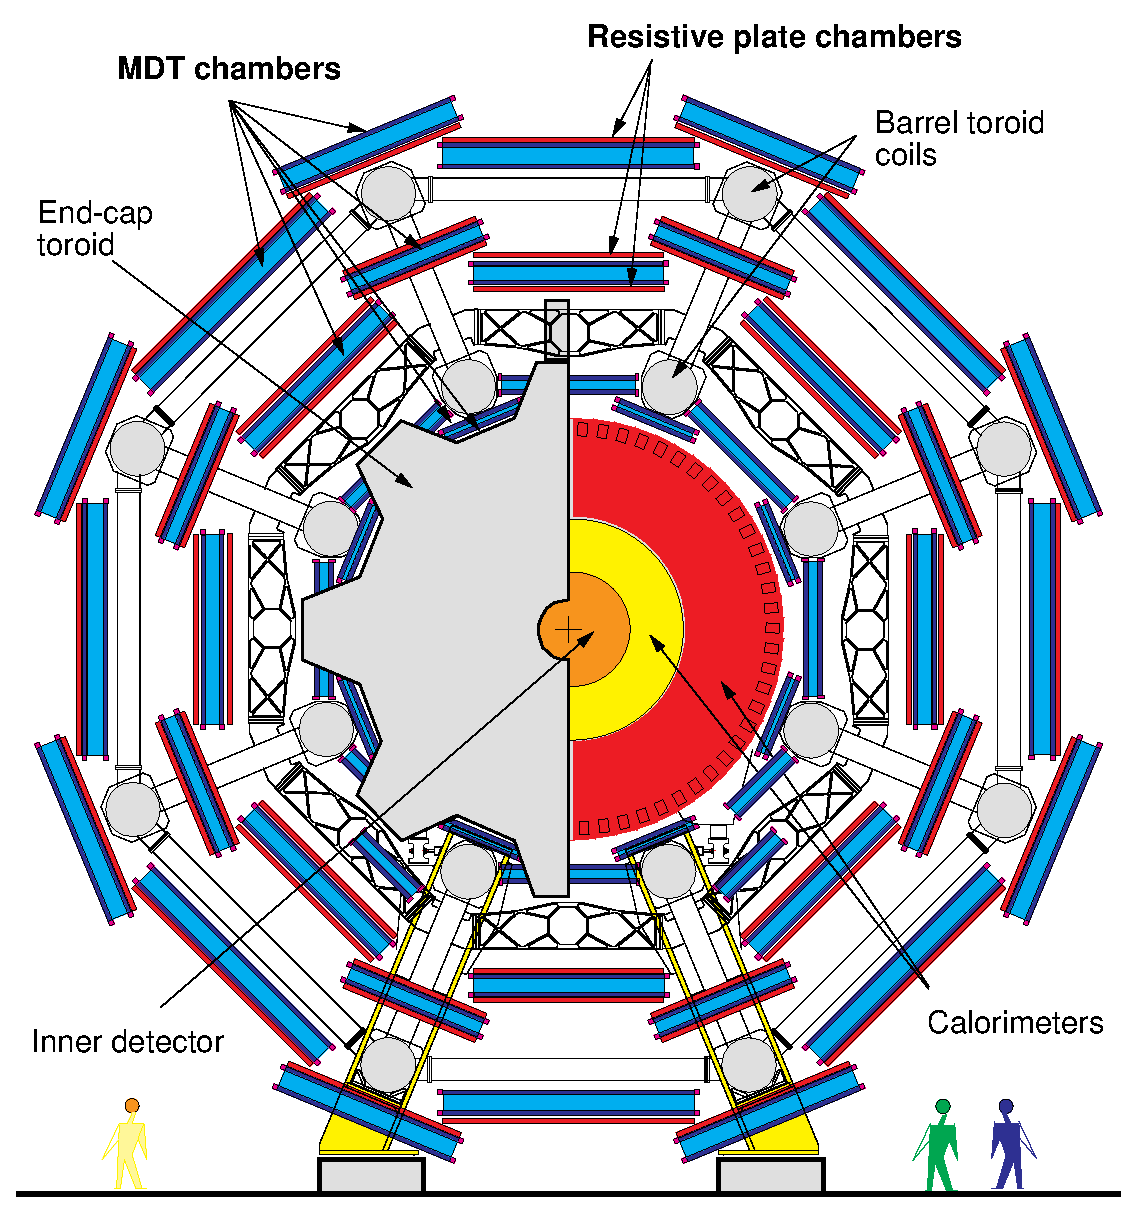
\includegraphics[width=0.5\textwidth]{figures/experiment/atlas/muonCross.eps}}}
\caption{}
\label{fig:atlasMs}
\end{figure}

The outermost detector system, the ATLAS Muon Spectrometer (MS), is the largest muon spectrometer ever constructed. \check
The MS is able to identify muons and measure their transverse momentum, especially for those with $\pt>300$~GeV.
In this task, it shares a similar geometry to the ID.
The spectrometer is comprised of a barrel region with cylindrical layers of detectors at radii of 5, 7.5, and 10~m.
The symmetrical end-cap regions consist of a four layers located at $z$ of 7, 10, 14, 21-23~m. 
All layers have 16-fold symmetry in azimuth.
The MS uses of four subsystems in different regions of pseudorapidity and for different tasks. 
To provide fast hits to the trigger system in order to identify events containing muons, the Resistive Plate Chambers operate in the barrel ($|\eta|<1.05$) and the Thin Gap Chambers operate in the end-cap wheel ($1.05<|\eta|<2.7$).
Precision tracking data for muons is provided by the Monitored Drift Rubes in the barrel ($|\eta|<2.7$) along with the Cathode Strip Chambers in the region from $2.0<|\eta|<2.7$.
The various systems are shown in Figure \ref{fig:atlasMs}.
\cite{muonTdr}

The MS is required to measure muon momentum with a resolution,
\begin{equation}\begin{split}
    \frac{\Delta \pt}{\pt}<1\times10^{-4}\times p/\text{GeV}.
\end{split}\end{equation} 
This requires hit locations to be measured with an accuracy of 50~\um.
Hits are registered using cylindrical coordinates in the $r-z$ plane.
The $z$ coordinate is measured in the barrel region, where the toroidal magnetic field bends muons in the longitudinal direction.
Meanwhile $r$ coordinate is measured in the end-caps, where magnetic field pushes muons in the radial direction. 


%%Muon
%The MDTs are single wire ($50\mu m$) drift tubes (aluminum, radius 30mm) filled with 7\% $CO_2$ and 93\% Ar gas.
%These tubes are arranged in multilayers of 3 or 4 layers of drift tubes.
%Multilayers are grouped together into chambers with two multilayers each.
%Together, the MDTs achieve a spatial resolution of $\approx80\mu m$ and a momentum resolution of 10\% at Pt=1TeV.
%The CSCs are multiwire proportional chambers with four $\eta$ layers and four $\phi$ layers of anodes.
%At their peak performance, the CSC have a resolution of $\approx60\mu$m.
%They are used in the high $\eta$ region where the particle rate ($>150 Hz/cm^2$) exceeds the tolerance of the MDTs.
%The RPCs provide the muon trigger and $\phi$ coordinates in the barrel region ($|\eta|<2.7$).
%These chambers consist of $\eta$ and $\phi$ planes of cathode and anode pads separated by a 2mm gas gap and a voltage gradient.
%The TGCs fill a role similar to the RPCs in the end-cap region ($|\eta|<1.05$).
%The TGCs are multiwire proportional chambers with several layers of $\eta$ and $\phi$ planes. \cite{det-muon}

\subsubsection{MDT} % precision

\begin{figure}[h!]
\captionsetup[subfigure]{position=b}
\centering
\subfloat[][]{\label{fig:atlasMdt}{\includegraphics[width=0.5\textwidth]{figures/experiment/atlas/mdt.png}}}
\subfloat[][]{\label{fig:atlasMdtChamber}{\includegraphics[width=0.5\textwidth]{figures/experiment/atlas/mdtChamber.png}}}
\caption{}
\label{fig:}
\end{figure}

The Monitored Drift Tubes (MDT) are the single wire chambers that provide precision muon measurements in the majority of the MS.
An MDT consists of a 30~mm aluminum tube cathode with a central 50\um gold-plated tungsten-rhenium wire anode.
The tube is filled with a mixture of argon (91\%), nitrogen (4\%), and methane (5\%) pressurized to 3~bar.
Charged particles passing through the tube ionize the gas, freeing a track electrons to drift towards the 3.2~kV wire over the course of $\approx500$~ns.
The spacial resolution of a single MDT is 80~\um.
This is shown in Figure \ref{fig:atlasMdt}.
The radial displacement of the track is determined from the total drift time.
Layers of MDTs are laminated together with glue and affixed to a support frame that holds them in precise positions.
This is shown in Figure \ref{fig:atlasMdtChamber}.
The central cross plate is adjustable to bend the outer aluminum tubes to match the gravitational sag of the anode wires.
The deformation of the chamber is monitored by built in optical systems.

As shown in Figure \ref{fig:atlasMs}, the MDT chambers are used throughout ATLAS except in the very high pseudorapidity region where particle flux exceeds their measurement rate.
In the barrel ($|\eta|<1$), chambers are rectangular and arranged into three layers beginning outside the calorimeters, as shown in Figure \ref{fig:atlasMsBarrel}.
In the end-cap ($|\eta|>1$), chambers are trapezoidal and positioned radially on either an inner or outer wheel.
The MDT system is comprised of 1194 precision chambers, with a total of 370,000 output channels.

\cite{muonTdr}

\subsubsection{CSC} % precision

\begin{figure}[h!]
\captionsetup[subfigure]{position=b}
\centering
\subfloat[][]{\label{fig:atlasCsc}{\includegraphics[width=0.5\textwidth]{figures/experiment/atlas/csc.png}}}
\caption{}
\label{fig:}
\end{figure}

The Cathode Strip Chambers (CSC) are multiwire proportional chambers that provide precision muon measurements in the region close to the interaction point and the beamline ($2<|\eta|<2.7$).
The CSCs are designed to have short drift times ($<30$~ns) in order to avoid saturation from the high particle flux in this region.
Like the MDTs, the spacial resolution of CSCs is 80~\um.
They consist of anode wires strung perpendicularly to cathode strips as shown in Figure \ref{fig:atlasCsc}.
The wires in the CSCs are 30~\um versions of those used in the MDTs, and the cathode strips are copper adhered to glass-reinforced epoxy.
Four of these constructions are stacked on top of each other, separated by a closed cell foam, to complete a CSC chamber.
The intermediate area is filled with a mixture of carbon dioxide (50\%), argon (30\%), and carbon tetrafluoride (20\%).

When an ionizing particle passes through the CSC, it produces an electron avalanche onto adjacent anode wires.
This induces a charge on the cathode strips, which in turn is amplified and read out.
Long cathode strips provide coarse information, while short segmented cathodes provide precision hit data.
The CSC system is comprised of 32 precision chambers, with a total of 67,000 output channels.
\cite{muonTdr}

\subsubsection{Trigger Chambers}

The MDT and CSC chambers are supported by additional types of chamber that provide rapid data for the trigger decision.
These are the Resistive Plate Chambers (RPC) in the barrel, and the Thin Gap Chambers (TGC) in the end-caps.
These are positioned in close proximity to a corresponding precision chamber.
The RPCs consist of two resistive plates coated in thin layers of graphite, held at 8.9~kV.
A 2~mm gap between the plates is filled with gas (tetrafluoroethane with 3\% isobutane).
An ionizing particle passing through the gap instigates an electron avalanche, which is read out by conductive strips on both sides of the gap.
The strips are orthogonal to each other.
Two RPC layers are combined in a station, separated by a 6~mm support.
The RPC system is comprised of 596 trigger chambers, with a total of 355,000 output channels.
The TGCs are multiwire proportional chambers with a small 2.8~mm gap.
The 50~\um anode wires are held at 3.1~kV, and the chamber is filled with carbon dioxide (55\%) and $n$-pentane (45\%).
The TGC system is comprised of 192 trigger chambers, with a total of 440,000 output channels.
\cite{muonTdr}

\subsection{Magnet System}

\begin{figure}[h!]
\captionsetup[subfigure]{position=b}
\centering
\subfloat[][]{{\includegraphics[width=0.5\textwidth]{figures/experiment/atlas/magnets.png}}}
\caption{{\color{red} Improve picture} Illustration of the geometry of the magnet system field coils. In the center, the Central Solenoid, surrounded by the eight windings of the Barrel Toroid. On opposing ends, the two pairs of eight windings make up the End-Cap Toroids. Figure from \cite{magnetTdr}.}
\label{fig:atlasMagnets}
\end{figure}

%magnet
The ATLAS Magnet System is composed of three superconducting magnet systems: the Central Solenoid, the Barrel Toroid, and the two End-Cap Toroids.
The arrangement of these magnets is shown in Figure \ref{fig:atlasMagnets}.
The purpose of these magnets is to produce a strong magnetic field to enable the measurement of momenta of charged particles.
Each coil that makes up the magnets is effected not only by gravity but also magnetic forces.
To support them, each coil is enclosed in a mechanical structure that also houses cooling circuits and cryostats to maintain their operating temperature of $\sim4.5$~K.
The coils are wound with superconducting niobium-titanium in a copper-aluminum matrix.
When the four magnets are fully energised, the magnet fields store an energy of 1.3 GJ. \footnote{This is equivalent to the energy released by an explosion of 300 kg of TNT}

The large Barrel Toroid (BT) magnet is one of the most visible features of the experiment.
The magnet is the largest in ATLAS and spans 26~m along the beamline with a diameter of 20~m. 
It consists of eight air-cooled coils surrounding parts of the muon spectrometer.
The coils each contain 120 turns, and the coils are wired in series.
At its strongest, the field of the BT reaches 3.9~T.
Finally two air-cooled End-Cap Toroids (ECT) provide a magnetic field for the MS wheels.
These have a length of 5~m and outer diameter of 10.7~m. An inner diameter of 1.65~m is left empty to allow passage of the beam.
Like the BT, both ECTs consist of eight coils, but with 116 turns.
All 16 ETC coils are wired together in series.
The fields of the ETC reach a peak of 4.1~T.
Both toroids are operated with a current of 20 kA.
Tubes carrying 4.5~K helium are welded onto the casings of the windings to keep them at superconducting temperatures.

The innermost magnet is the cylindrical Central Solenoid (CS), which is 5.3~m long and 2.4~m in diameter.
The CS produces a magnetic field of 2.0-2.6~T in the region of the inner detector.
The coil consists of a single layer coil wound 1173 times around a cylinder.
In order to reduce the amount of material that particles can interact with in the inner detector, the CS shares a vacuum vessel and cryostat with the Liquid Argon Calorimeter.
\cite{atlasFacts}
\cite{magnetTdr}

\subsection{Trigger System}

\begin{figure}[h!]
\captionsetup[subfigure]{position=b}
\centering
\subfloat[][]{{\includegraphics[width=0.5\textwidth]{figures/experiment/atlas/trigger.png}}}
\caption{}
\label{fig:atlasTrigger}
\end{figure}

The nominal 24.96~ns bunch spacing for LHC beams results in 40 million bunch crossings per second.
A beam with a luminosity of $1.5\times10^{34}$\cms produces approximately 30 collisions per bunch crossing.
This results in approximately 1.2 billion collisions per second.
During operation data is read from approximately one hundred million electronic output channels across approximately three million meters of cables. \cite{atlasFacts}
The data recorded from a typical event is 1.5~MB, resulting in 156~EB worth of data generated by ATLAS per day.
\footnote{For comparison, this is a sizable fraction of humanity's existing storage and roughly 30,000 times the total data collected by the Event Horizon Telescope.}
The Trigger System is responsible for rapidly sorting through this data and selecting events to record and events to discard.
It takes hit information from the ID, MS, and calorimeters and searches for signatures of interesting collisions.
The trigger decision is made by computers in the nearby underground service area (USA15), so data must first be transmitted to these.
A schematic of the trigger system is shown in Figure \ref{fig:atlasTrigger}.

The first rejection of events reduces the event rate from $\approx1.2$~GHz to $\approx100$~MHz is performed by the Level-1 (L1) Trigger.
This selects searches for the signatures of interesting particles (high-\pt muons, electrons, jets and others) in a subset of the detectors.
When an event passes the L1 Trigger, it sends an ``accept'' signal is sent back to the detector.
Meanwhile, various front-end electronics have stored precision hit data.
When they receive a L1 accept, they transmit this data off the detector to USA15.
Since the front-end electronics must store hit information while waiting for a possible L1 Trigger decision, the target time frame for this is 2~\us. 
\cite{triggerTdr}

The data is sent from the detector into \emph{readout buffers} (ROB) for temporary storage while the Level-2 (L2) Trigger evaluates the event with a broader set of criteria.
The L2 trigger reduces the event rate down to $\approx1$~kHz.
It works by searching \emph{regions-of-interest} (ROI) constructed by the preliminary L1 trigger information.
Based on the $\eta-\phi$ location of the ROI, the trigger logic accessed the precision data stored in the ROBs.
This process takes longer than the L1 decision, on the order of 10~ms.
With the precision data available, the L2 trigger can make strict requirements on the kinematics of various objects.
For example, this analysis uses muon and electron triggers that require leptons passing certain thresholds of \pt or \et, respectively.
Events passing the L2 trigger are passed along for full reconstruction.
The fully reconstructed events are filtered by the Event Filter, which reduces the rate down to  $\approx$100~Hz.
\cite{triggerTdr}
